\chapter{Brief Description of Mancala Game}
%Begin from here
It’s a board two-player game. The board is partitioned into 14 holes. Each player has 6 holes in front of
them and a single hole for their score. Each player needs to collect as many stones as they
can in their score hole to win the game.

\chapter{How did we implement the game?}
We implemented each state of the game (number of stones in each hole) with a python tuple where tuple[0] is 
an array modeling the state of the board and the tuple[1] is the index of the hole played to get to
that state. 
\vskip 0.25in

\chapter{Utility Functions}
\begin{enumerate}
    \item print\_board(state) :
    \begin{itemize}
        \item prints the board to console based on passed state.
    \end{itemize}
    \item let\_user\_player() :
    \begin{itemize}
        \item allows the system to get user play.
    \end{itemize}
    \item convert\_play\_to\_state(previous\_state, play) : 
    \begin{itemize}
        \item takes the state and the play chosen by human ,then convert the state to the new state according to the human play.  
    \end{itemize}
    \vskip 0.5in
    \item get\_node\_children(in\_state: list, stealing=True/False):  
    \begin{itemize}
    \item it takes the current state of the game, and then calculating each possible state that can be
     got into from that current state (children of current state). Optional argument “stealing” if you 
     pass it with true then stealing mode is activated, else its without stealing.
    \end{itemize}
    \vskip 0.1in
    \item evaluate(state)  :
    \begin{itemize}
        \item evaluates the state by subtracting the number of stones in each side and the best state
         is the one that keeps your stones as much as possible.  
    \end{itemize}
    \item possibleMoves(state) :
    \begin{itemize}
        \item returns all possible plays that each player can play. In other words excludes
         the zero play (playing a hole which has no stones).
    \end{itemize}



    \item extra\_turn(state, selected\_hole, player\_type)   :
    \begin{itemize}
        \item checks if the player has to play again (the case when the last stone is
          dropped in the score hole).
    \end{itemize}



    \item is\_game\_over(state)    :
    \begin{itemize}
        \item checks if the game is over by checking if there is a whole side with no stones.
    \end{itemize}


    \item who\_wins(state)     :
    \begin{itemize}
        \item checks who wins by subtracting the stones of each player and whoever has more stones wins.
    \end{itemize}


    
\end{enumerate}       




\chapter{A user guide with snapshots}
You can play our game by first cloning our repository\url{https://github.com/Mohammed-Hussien/Mancala_Ai.git}. 
use the command git clone to clone the repo.

\begin{figure}[H]
    \centering
    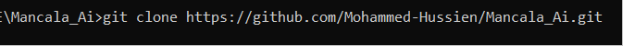
\includegraphics[width=100mm,height=10mm]{Images/git_clone.png}
    \caption{cloning the repo}
  \end{figure}
  \vskip 0.2in
\vskip 0.2in
You will find a file called mancala.exe, just run that file and enjoy!




\chapter{Task Breakdown}

\begin{enumerate}
    \item Mohamed Hussien Mostafa Masaoud:
    \begin{itemize}
        \item MiniMax  Algorithm Implementation, Integration and game loop.
    \end{itemize} 
    \vskip 0.2in
    \item Mohamed Emad Mahmoud Abd Al Hamid:
     \begin{itemize}
        \item AlphaBeta  Algorithm Implementation, Integration and game loop.
    \end{itemize}
    \item Mohamed Amr Ahmed Taha:
    \begin{itemize}
        \item Utility functions: who wins, is\_game\_over, convert\_paly\_to\_state, evaluate, possible\_moves.
    \end{itemize} 
    \item Mohamed Amr Mohamed Hassan:
    \begin{itemize}
        \item Utility functions: extra\_turn, possible\_moves, Integration and game loop.
    \end{itemize}
    \item Mohamed Khaled Rashad:  
   \begin{itemize}
        \item Utility functions: get\_node\_children, print\_board, Integration and game loop.
    \end{itemize}
\end{enumerate}